% IEEE standard conference template; to be used with:
%   spconf.sty  - LaTeX style file, and
%   IEEEbib.bst - IEEE bibliography style file.
% --------------------------------------------------------------------------

\documentclass[letterpaper]{article}
\usepackage{spconf,amsmath,amssymb,graphicx,hyperref}
\graphicspath{{figures/}}

% Example definitions.
% --------------------
% nice symbols for real and complex numbers
\newcommand{\R}[0]{\mathbb{R}}
\newcommand{\C}[0]{\mathbb{C}}

% bold paragraph titles
\newcommand{\mypar}[1]{{\bf #1.}}

% Title.
% ------
\title{Parallel Implementation of Breadth-First Search}
%
% Single address.
% ---------------
\name{Markus P\"uschel\thanks{The author thanks Jelena Kovacevic. This paper
is a modified version of the template she used in her class.}} 
\address{Department of Computer Science\\ ETH Z\"urich\\Z\"urich, Switzerland}

% For example:
% ------------
%\address{School\\
%		 Department\\
%		 Address}
%
% Two addresses (uncomment and modify for two-address case).
% ----------------------------------------------------------
%\twoauthors
%  {A. Author-one, B. Author-two\sthanks{Thanks to XYZ agency for funding.}}
%		 {School A-B\\
%		 Department A-B\\
%		 Address A-B}
%  {C. Author-three, D. Author-four\sthanks{The fourth author performed the work
%		 while at ...}}
%		 {School C-D\\
%		 Department C-D\\
%		 Address C-D}
%




\begin{document}
%\ninept
%
\maketitle
%

The hard page limit is 6 pages in this style. Do not reduce font size
or use other tricks to squeeze. This pdf is formatted in the American letter format, so the spacing may look a bit strange when printed out.


% TODO
\begin{abstract}
Describe in concise words what you do, why you do it (not necessarily
in this order), and the main result. The abstract has to be
self-contained and readable for a person in the general area. You
should write the abstract last.
\end{abstract}



\section{Introduction}\label{sec:intro}

%Do not start the introduction with the abstract or a slightly modified
%version. It follows a possible structure of the introduction. 
%Note that the structure can be modified, but the
%content should be the same. Introduction and abstract should fill at most the first page, better less.

\mypar{Motivation}
%The first task is to motivate what you do.  You can
%start general and zoom in one the specific problem you consider.  In
%the process you should have explained to the reader: what you are doing,
%why you are doing, why it is important (order is usually reversed).
%
%For example, if my result is the fastest sorting implementation ever, one
%could roughly go as follows. First explain why sorting is important
%(used everywhere with a few examples) and why performance matters (large datasets,
%realtime). Then explain that fast implementations are very hard and
%expensive to get (memory hierarchy, vector, parallel). 
%
%Now you state what you do in this paper. In our example: 
%presenting a sorting implementation that is
%faster for some sizes as all the other ones.
Breadth-first search is a graph traversing algorithm which is used in many applications. Some examples are finding connected components, determining a shortest-path for navigation systems or computing the maximum flow in a network. As real-world graphs can get very large, for example the US road network graph contains roughly 24 million vertices and 57 million edges, the need for fast implementations is high.

In this paper, we will discuss multiple approaches and compare their performance on three different platforms.

\mypar{Related work} 
%Next, you have to give a brief overview of
%related work. For a report like this, anywhere between 2 and 8
%references. Briefly explain what they do. In the end contrast to what
%you do to make now precisely clear what your contribution is.
In this section we will give a brief overview of related work. In the first part we will discuss the work covering the top-down-bottom-up hybrid approach and in the second part an approach that focuses on avoiding atomic operations.

% Hybrid:
\cite{6691600}
\cite{beamer2011searching}

% Avoid atomic
Berrendorf \cite{Berrendorf:14} describes a technique to avoid atomic operations in a generalized scenario. The scenario is given as an if-statement followed by some operations that change a state, where multiple threads might execute the predicate and execute the operations afterwards. The operations need to change the state to the same value if executed multiple times otherwise there exists a race condition, i.e. the change of the distance of a visited vertex to the value of the level or the addition of a vertex to the next frontier. The trade-off is that doing a BFS this way can result in additional work any unvisited vertex may get added multiple times.



% TODO
\section{Background: Whatever the Background is}\label{sec:background}

Give a short, self-contained summary of necessary
background information. For example, assume you present an
implementation of sorting algorithms. You could organize into sorting
definition, algorithms considered, and asymptotic runtime statements. The goal of the
background section is to make the paper self-contained for an audience
as large as possible. As in every section
you start with a very brief overview of the section. Here it could be as follows: In this section 
we formally define the sorting problem we consider and introduce the algorithms we use
including a cost analysis.

fmypar{Sorting}
Precisely define sorting problem you consider.

\mypar{Sorting algorithms}
Explain the algorithm you use including their costs.

As an aside, don't talk about "the complexity of the algorithm.'' It's incorrect,
problems have a complexity, not algorithms.



% TODO
% hybrid: doing topdown or bottum up, depending on heuristic switch. uses 1x OMP critical section in topdown part and localneighbourhoods + prefix sum to add them together at each level in the bottom up part. Idea from paper by Yasui et al
% nonlevel: using 1xCAS to check visited and  1xOMP critical for the distance update (needs to see if unvisited or visited from further away), frontier is a single queue. if a thread finishes with his part he waits for the others to finish (no loadbalancing). Idea from talking with Timo.
% nonlevel with work stealing. Idea is for threads that are finished with their part to steal work from a randomly choosen other thread. Only works with too much synchronization (slow) at the moment. Idea from talking with Timo.

\section{Your Proposed Method}\label{sec:yourmethod}

%Now comes the ``beef'' of the report, where you explain what you
%did. Again, organize it in paragraphs with titles. As in every section
%you start with a very brief overview of the section.
%
%In this section, structure is very important so one can follow the technical content.
%
%Mention and cite any external resources that you used including libraries or other code.

We implemented many different algorithms and multiple variants for most of them. They return a distance map from one source vertex to all reachable vertices in the graph.

All our implementations are based on OpenMP for synchronization.


\mypar{Topdown}
A lot of our approaches are based on a simple topdown algorithm. The idea is to do a level-synchronous traversal of the graph by keeping record of the vertices in the current as well as those in the next level (``frontier'' and ``neighbour'') in two data structures of the same type and setting the frontier to the current neighbours after each level. This leads to an implicit barrier, as the work done by the different threads has to be synchronized. We experimented with different data structures and synchronization methods.

% naive
% using 1x OMP critical section (check visited and add to frontier), frontier is a vector to allow easy dynamic splitting after each level (load balancing between threads). basically naive implementation
The naive version of the topdown algorighm has a global standard vector for the frontier to allow easy dynamic splitting between the threads in each level. This balances the load between treads, however it has a significant overhead because it relies on a critical section (\verb+OMP critical+) for checking whether the vertices were already visited and inserting them into the neighbour data structure.

% topdownCAS
% using CAS (check visited) + OMP critical section (add to frontier), also vector frontier. Idea from paper by Berrendorf
To improve the naive implementation, we used atomics, the built-in \verb+__sync_val_compare_and_swap+ to atomically check whether a vertex was visited and set the correct distance. It also uses a local neighbourhood data structure (standard vector) to prevent needing a critical section. Only at the end of each level, a lock (\verb+omp_lock_t+) is used to combine the local neighbourhoods to a global one, which can then be distributed between the threads for the next level. This is an idea adapted from Berrendorf \cite{Berrendorf:14}.

% topdown_ifCAS
% same as topdownCAS but doing a nonatomic visited check before each CAS, Idea from paper by Berrendorf
An extended version of the algorithm before first uses a non-atomic check if a vertex visited before each CAS.

% topdown_nonatomic
% doing the visited check nonatomic (adds additional work but no race condition), using localneighbourhood and OMP lock to add them to the global neighbourhood after a thread has looked at all neighbours from one node. Idea from paper by Berrendorf
Also inspired by Berrendorf \cite{Berrendorf:14} is the idea to remove atomics alltogether. This results in a race condition where additional work for the next is created, as some vertices might be added to the neighbours multiple times. However, expensive atomics are omitted, which results in a trade-off between the additional time from the added work and the faster runtime by leaving out the CAS. This algorithm still uses a local neighbourhood and a lock when combining them.

% parallelbfs1
% using 3x bool arrays for visited, looping over all nodes on each level, frontier is a mask
Instead of using a standard vector for the frontier and the neighbour, one of our implementation relies on a bool array for all data structures (visited vertices, frontier, neighbour). This makes it possible to remove all critical sections, as the insertion of an element into a vector was what made them necessary in the first place. Similarly to the algorithm before, there might be additional work due to avoiding atomics. The downside of this implementation is that in each level, you have to loop through all the vertices, not just the current frontier, to be able to explore from there. Depending on the structure of the graph, this can be much more work.

% TODO
% tbb_parallelqueue
% doing a topdown method using 1x OMP single for level synchronization and TBB concurrentqueue as a concurrent frontier

% even_odd_parallelqueue
% using only implicit OMP barrier for level synchronization. switching between two TBB parallelqueue frontiers




\section{Experimental Results}\label{sec:exp}

Here you evaluate your work using experiments. You start again with a
very short summary of the section. The typical structure follows.

\mypar{Experimental setup}
%Specify the platform (processor, frequency, maybe OS, maybe cache sizes)
%as well as the compiler, version, and flags used. If your work is about performance, 
%I strongly recommend that you play with optimization flags and consider also icc for additional potential speedup.
%
%Then explain what kind of benchmarks you ran. The idea is to give enough information so the experiments are reproducible by somebody else on his or her code.
%For sorting you would talk about the input sizes. For a tool that performs NUMA optimization, you would specify the programs you ran.
We run experiments on three different platforms.

The first platform is the EULER cluster which is operated by the HPC Group of ETH. We had access to one node with a 12-core Intel Xeon E5-2697v2 processors (2.7 GHz nominal, 3.0-3.5 GHz peak). It supports hyper-threading, so we ran our algorithms with up to 24 threads. On this platform, we used the gcc compiler with the -O2 flag.

The next platform we ran our algorithms on is the Xeon Phi provided through the class.

Lastly, we also used an AMD FX-8350 (4GHz x8, 8Gb, W2k3).

% TODO
\mypar{Results}
Next divide the experiments into classes, one paragraph for each. In each class of experiments you typically pursue one questions that then is answered by a suitable plot or plots. For example, first you may want to investigate the performance behavior with changing input size, then how your code compares to external benchmarks.

For some tips on benchmarking including how to create a decent viewgraph see pages 22--27 in



{\bf Comments:}
\begin{itemize}
\item Create very readable, attractive plots (do 1 column, not 2 column plots
for this report) with readable font size. However, the font size should also not be too large; typically it is smaller than the text font size.
An example is in Fig.~\ref{fftperf} (of course you can have a different style).
\item Every plot answers a question. You state this question and extract the
answer from the plot in its discussion.
\item Every plot should be referenced and discussed.
\end{itemize}

\begin{figure}\centering
  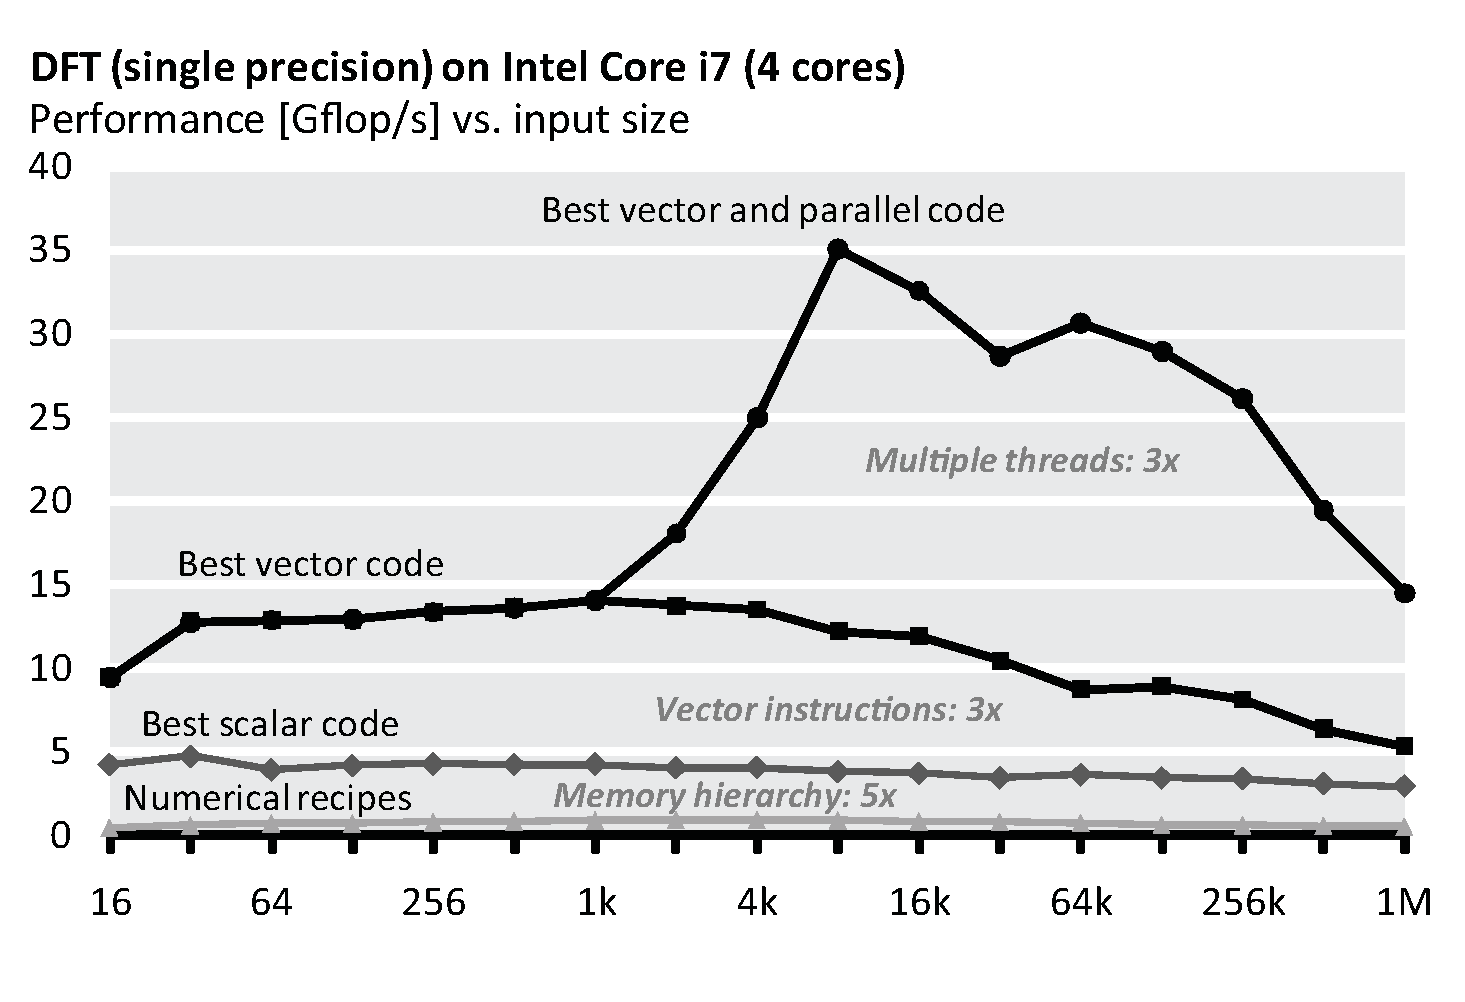
\includegraphics[scale=0.33]{dft-performance.eps}
  \caption{Performance of four single precision implementations of the
  discrete Fourier transform. The operations count is roughly the
  same. The labels in this plot are maybe a little bit too small.\label{fftperf}}
\end{figure}



% TODO
\section{Conclusions}

Here you need to summarize what you did and why this is
important. {\em Do not take the abstract} and put it in the past
tense. Remember, now the reader has (hopefully) read the report, so it
is a very different situation from the abstract. Try to highlight
important results and say the things you really want to get across
such as high-level statements (e.g., we believe that .... is the right
approach to .... Even though we only considered x, the
.... technique should be applicable ....) You can also formulate next
steps if you want. Be brief. After the conclusions there are only the references.



% TODO
\section{Further comments}

Here we provide some further tips.

\mypar{Further general guidelines}

\begin{itemize}
\item For short papers, to save space, I use paragraph titles instead of
subsections, as shown in the introduction.

\item It is generally a good idea to break sections into such smaller
units for readability and since it helps you to (visually) structure the story.

\item The above section titles should be adapted to more precisely
reflect what you do.

\item Each section should be started with a very
short summary of what the reader can expect in this section. Nothing
more awkward as when the story starts and one does not know what the
direction is or the goal.

\item Make sure you define every acronym you use, no matter how
convinced you are the reader knows it.

\item Always spell-check before you submit (to us in this case).

\item Be picky. When writing a paper you should always strive for very
high quality. Many people may read it and the quality makes a big difference.
In this class, the quality is part of the grade.

\item Books helping you to write better:

\item Conversion to pdf (latex users only): 

dvips -o conference.ps -t letter -Ppdf -G0 conference.dvi

and then

ps2pdf conference.ps
\end{itemize}

\mypar{Graphics} For plots that are not images {\em never} generate the bitmap formats
jpeg, gif, bmp, tif. Use eps, which means encapsulate postscript. It is
scalable since it is a vector graphic description of your graph. E.g.,
from Matlab, you can export to eps.

The format pdf is also fine for plots (you need pdflatex then), but only if the plot was never before in the format 
jpeg, gif, bmp, tif.





% References should be produced using the bibtex program from suitable
% BiBTeX files (here: bibl_conf). The IEEEbib.bst bibliography
% style file from IEEE produces unsorted bibliography list.
% -------------------------------------------------------------------------
\bibliographystyle{IEEEbib}
\bibliography{bibl_conf}


\end{document}

